\begin{frame}[allowframebreaks]{Neural Network Types}
    \begin{figure}
        \centering
        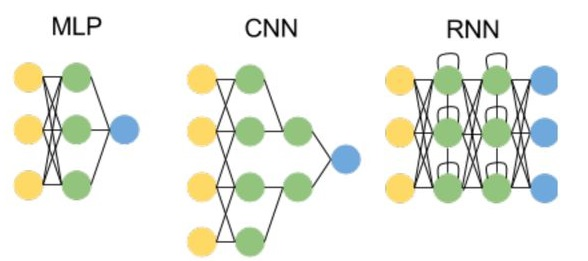
\includegraphics[width=1\textwidth,keepaspectratio]{images/rnn/slide_2_1_img.jpg}
    \end{figure}
\end{frame}


\begin{frame}[allowframebreaks]{Recurrent Neural Networks (RNN)}
    \begin{columns}
    \begin{column}{0.5\textwidth}
        \begin{figure}
            \centering
            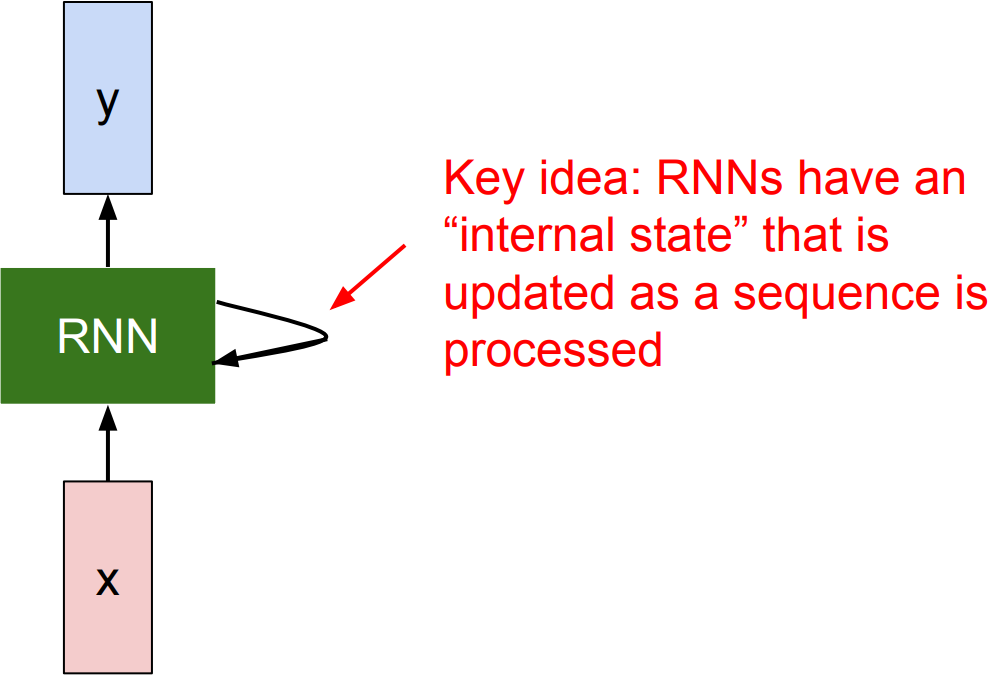
\includegraphics[width=1.05\textwidth,keepaspectratio]{images/rnn/slide_3_1_img.png}
        \end{figure}
    \end{column}
    \begin{column}{0.5\textwidth}
        \begin{figure}
            \centering
            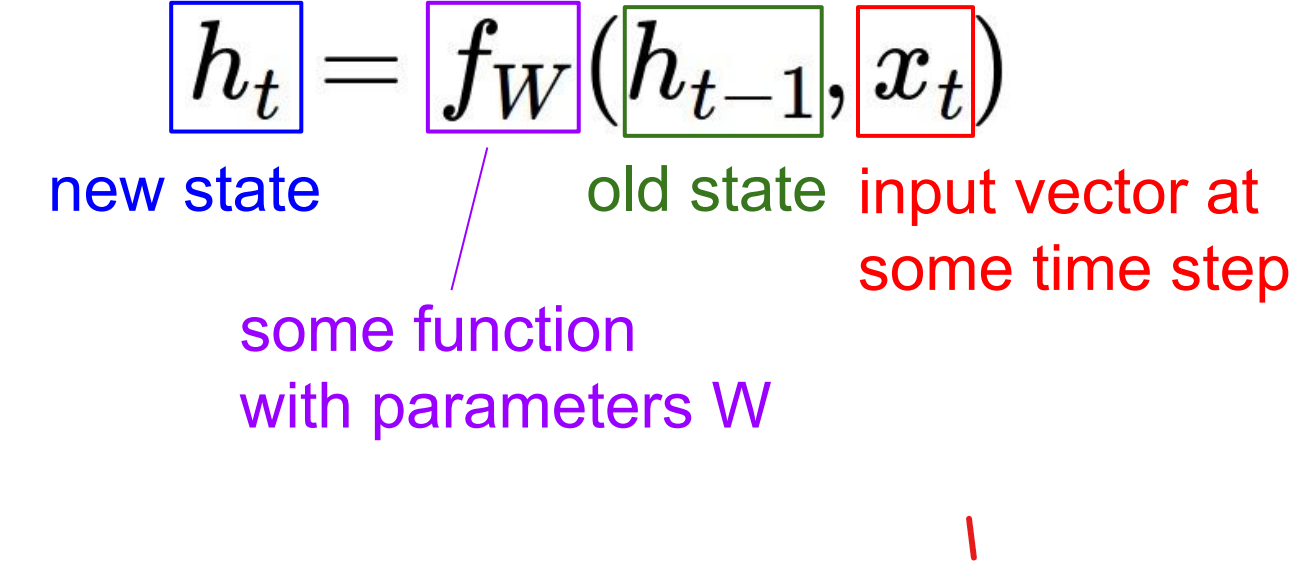
\includegraphics[width=1.05\textwidth,keepaspectratio]{images/rnn/slide_3_2_img.png}
        \end{figure}
    \end{column}
    \end{columns}

    \framebreak

    \begin{figure}
        \centering
        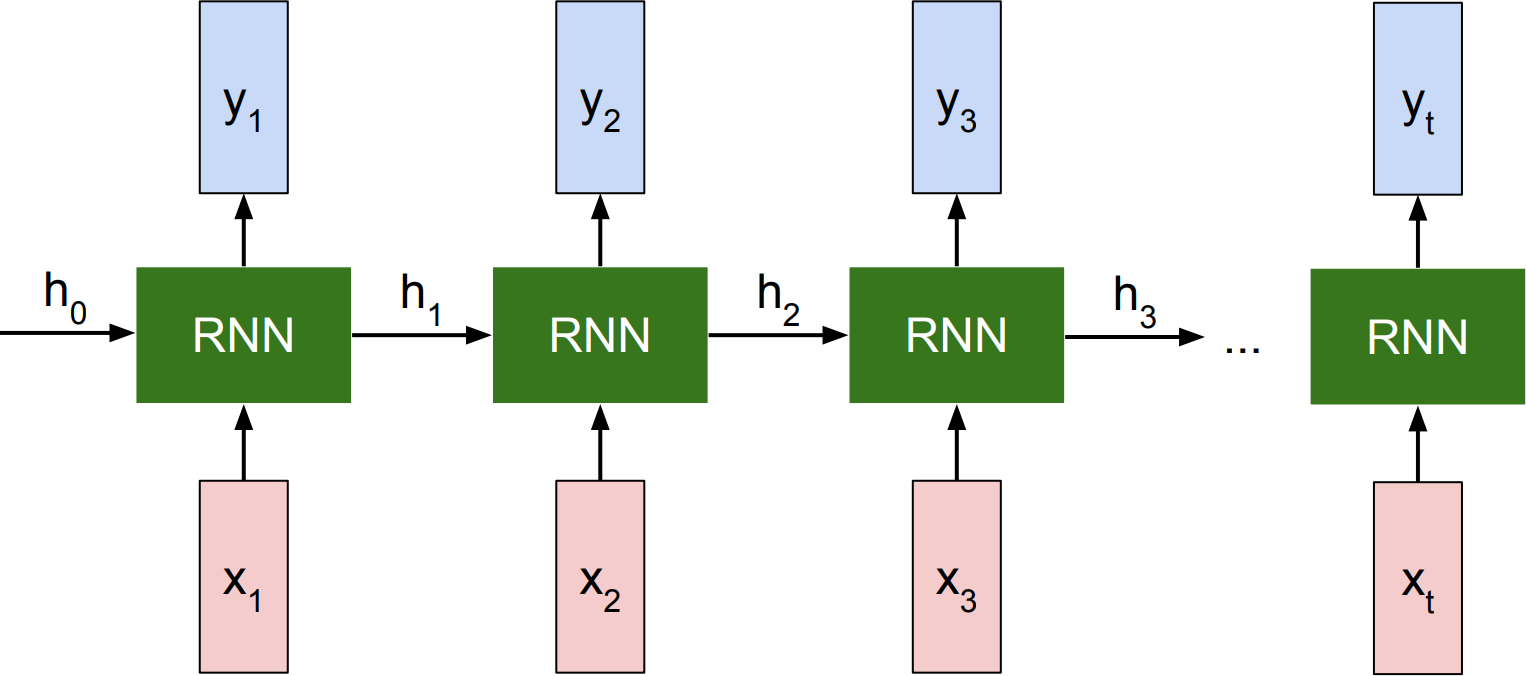
\includegraphics[width=1.05\textwidth,keepaspectratio]{images/rnn/slide_4_1_img.png}
    \end{figure}

    \framebreak

    \begin{figure}
        \centering
        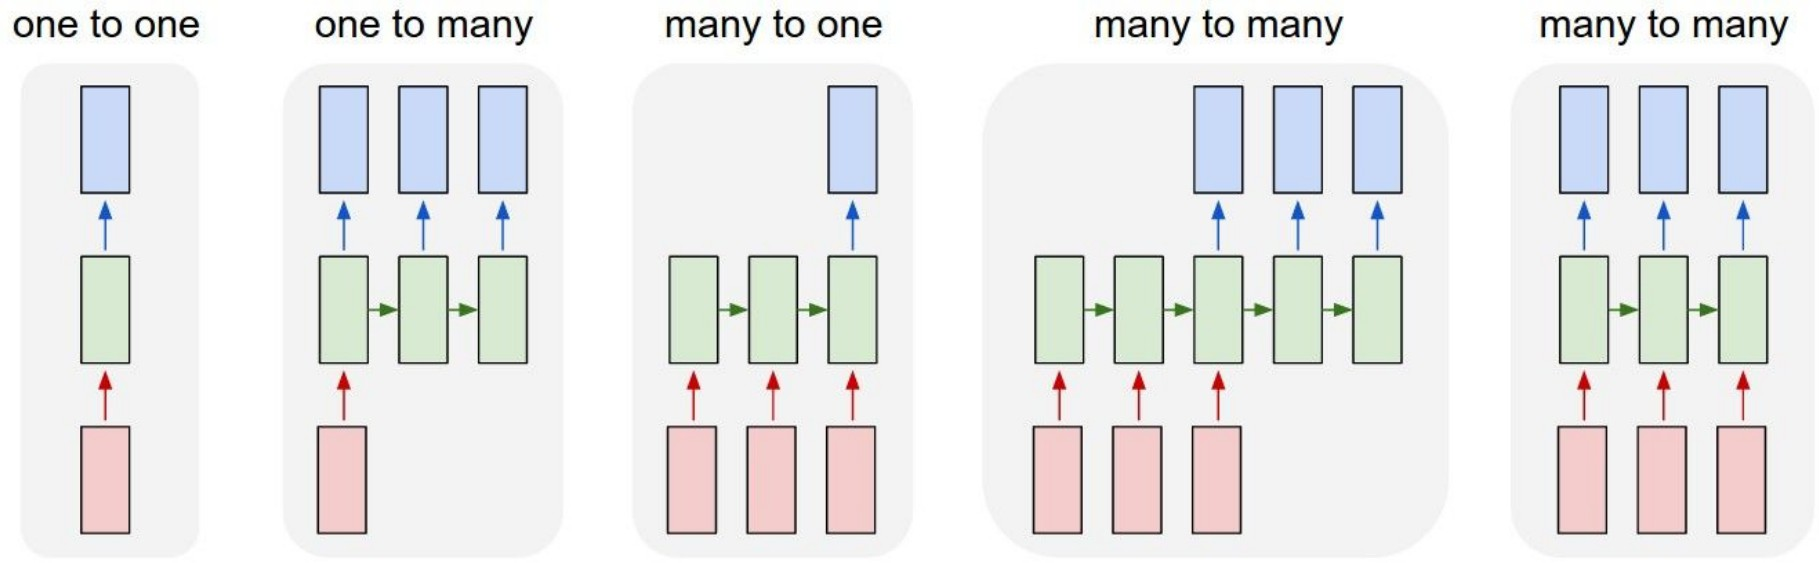
\includegraphics[width=1.05\textwidth,keepaspectratio]{images/rnn/slide_5_1_img.jpg}
    \end{figure}

    \framebreak

    \textbf{RNN Advantages:}
    \begin{itemize}
        \item Can process input sequences of any length.
        \item Computation at each time step can, in theory, utilize information from many previous steps.
        \item Model size remains constant regardless of input length.
        \item The same weights are applied at every time step, ensuring symmetry in input processing.
    \end{itemize}

    \vspace{1em}

    \textbf{RNN Disadvantages:}
    \begin{itemize}
        \item Recurrent computation is slow.
        \item In practice, difficult to access information from many steps back.
    \end{itemize}

\end{frame}